%%%%%%%%%%%%%%%%%%%%%%%%%%%%%%%%%%%%%%%%%%%%%%%%%%%%%%%%%%%%%%%%%%%%%%%%%%%%%%%%
%2345678901234567890123456789012345678901234567890123456789012345678901234567890
%        1         2         3         4         5         6         7         8

\documentclass[letterpaper, 10 pt, conference]{ieeeconf}  % Comment this line out if you need a4paper
\usepackage{graphicx}
\usepackage{url}
\usepackage{multirow}
\usepackage{array}
%\documentclass[a4paper, 10pt, conference]{ieeeconf}      % Use this line for a4 paper

\IEEEoverridecommandlockouts                              % This command is only needed if
                                                          % you want to use the \thanks command

\overrideIEEEmargins                                      % Needed to meet printer requirements.



% See the \addtolength command later in the file to balance the column lengths
% on the last page of the document

% The following packages can be found on http:\\www.ctan.org
%\usepackage{graphics} % for pdf, bitmapped graphics files
%\usepackage{epsfig} % for postscript graphics files
%\usepackage{mathptmx} % assumes new font selection scheme installed
%\usepackage{times} % assumes new font selection scheme installed
%\usepackage{amsmath} % assumes amsmath package installed
%\usepackage{amssymb}  % assumes amsmath package installed

\title{\LARGE \bf
Generator for Academic Reports: Abstracts
}




\author{
	\begin{tabular}{*{2}{>{\centering}p{.5\textwidth}}}
		\large Daniel Christiani & \large Cody Smith \tabularnewline
		Computer Engineering & Computer Engineering \tabularnewline
		Rochester Institute of Technology & Rochester Institute of Technology \tabularnewline
		\url{dmc3413@rit.edu} & \url{cds7494@rit.edu}
	\end{tabular}
}


\begin{document}
\maketitle

\begin{abstract}
	Academic reports are extremely important and often serious documents. They report findings in an organized and referenceable way to inform, record, and shape our understanding of our world. For each domain of study, there are common structures in syntax and overall semantic flow of the article, specifically in the abstract. For this reason we will attempt to do a meta-analysis of academic papers and their abstracts in an effort to uncover the underlying semantic structure, syntactic preferences, and vocabulary of a given sub-domain and author of an academic community by designing an algorithm to generate new abstracts for reports given a training set.
\end{abstract}


\section{Introduction}

In this paper we describe an approach to generate academic report abstracts, given a corpus of abstracts to learn from.  The training abstracts are used to generate convincing academic abstracts for a given domain via an algorithm implemented in python. The algorithm uses a variety of natural language techniques including context-free grammar, n-gram analysis, and grammar equivalency to fill in a predetermined learned structure for an abstract in that domain. Related works include the SCIgen automatic computer science paper generator, which has successfully generated papers which were accepted at several conferences at the expense of organizers.

\section{Corpora}

To create a successful system, first corpora of different domain's abstracts needed to be created. For our purposes, it was important that the reports were sorted by domain, and that the topics of the papers were similar. While many different options were considered, to manage the data in a straight-forward manager, the abstracts were copied out of reports that were manually copied into plain text files. The directory structure for our corpus is shown in Figure \ref{fig:Directorystructure}.

\begin{figure}[!ht]
	\centering
	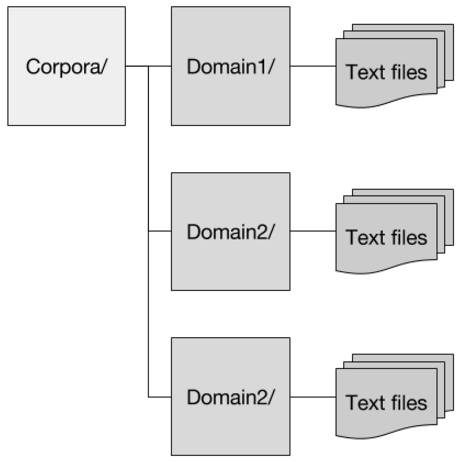
\includegraphics[width=.4\textwidth]{filestruct}
	\caption{Directory structure for the corpora.}
	\label{fig:Directorystructure}
\end{figure}

When accessing data from a corpus is required, the operation is as simple as looping over that directory and extracting the text from the text file. The code for doing that is shown in Figure \ref{fig:Codeparse}. Any additional corpus added to a domain directory will automatically be processed as additional data.

\begin{figure}[!ht]
	\begin{verbatim}
	data = ""
	full_path = os.getcwd() + path
	for i in os.listdir(full_path):
	if i.endswith(".txt"):
	with open(full_path + '/' + i, 'r')
	as f:
	data += f.read().replace('\n', ' ')
	\end{verbatim}

	\caption{Code to parse corpus.}
	\label{fig:Codeparse}
\end{figure}

We created three total corpora, each for a different domain of different sizes and from different sources. Are hope was that by having different domains, sizes, and sources we would be able to evaluate our solution easier and that their differences would expose flaws or sucesses in the system.

\subsection{Computer Science Corpus}

The computer science corpus is a collection of 24 computer science paper abstracts. These were taken from the 2015 publications from Carnagie Mellon University (CMU), ranging from identifier CMU-CS-15-100 and on. Besides their shared domain, the authors and topics vary from papers about searching algorthms, statistics, vertual machines and more.

\subsection{Linguistics Corpus}

The linguistics corpus is a collection of 17 abstracts from mendeley.com, tagged with the topic linguistics. The filenames in the corpora folder are the ISSN. Besides the shared linguistics tag, each of the abstracts do not share authors or topics. The topics range from lexical semantics, speech and pronounciation, linguistic universals, visualizing linguistic data, and more.

\subsection{Nanocomputing Corpus}

The nanocomputing corpus is a collection on 13 abstracts from found Google scholar with MORE INFORMATION HERE.

\section{Solution Overview}

The algorithm we developed is broken into three major parts. These parts include preprocessing, sentence generation, and scoring. An overview of each of these three steps is shown as Figure \ref{fig:SolutionOverview}.

\begin{figure}[!ht]
	\centering
	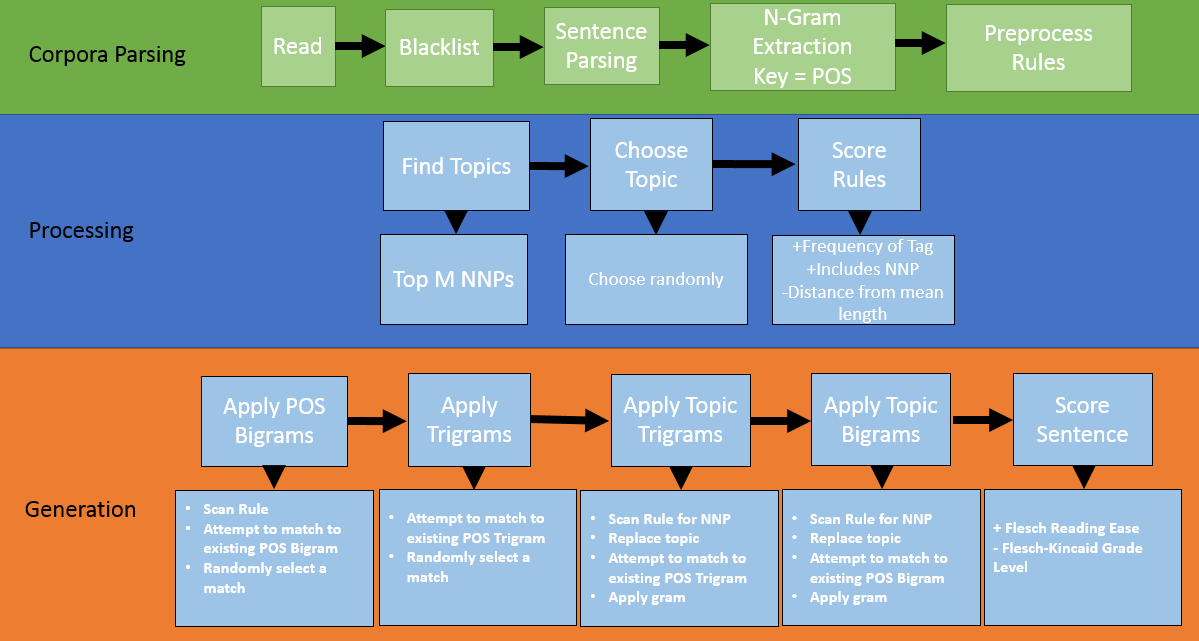
\includegraphics[width=.4\textwidth]{overall_flow}
	\caption{Directory structure for the corpora.}
	\label{fig:Directorystructure}
\end{figure}

\subsection{Preprocessing}

The first step in the preprocessing loads the text from a single corpus directory. For instance, choosing the directory ‘/computer_science’ will only load abstracts from the ‘Computer Science’ topic from which to preprocess text and eventually train our generator. Each line is read and the newline characters are stripped such that text will only be contiguous sentences.

Once the read is complete, the raw text is stripped of all text in a blacklist. This blacklist contains characters such as quotes, parenthisis, and commas. Manual inspection of the text proved the blacklist to be critical to guarantee no unwanted special characters were included in the final data. It was decided to use a blacklist instead of a whitelist because minus a couple of problematic characters, most punctuation seems to be valuble or at least has no negative consiquence to the final result.

After the data is read in and the blacklist is stripped out, sentences are parsed. The parser moves over the text tokenizing every word and placing them into a list associated with a unique sentence. Decimal valued numbers are are found first with a regular expression, and are treated as individual tokens, otherwise, a string containing a period ‘.’ is considered the last word in the current sentence. The period is finally stripped from the sentence as clean tokenized words will be associated with our vocabulary. Future revisions may capture a variety of honorifics (e.g. ‘Dr.’) along associated with names of people as single tokens, however this is currently not supported.

The preprocessing of the raw data is now complete, however we must store this data in a way that we can utilize a form of context free grammar (CFG). The preprocessing stage stores parts-of-speech tags of the cleaned sentences, parts-of-speech tags of the vocabulary in a dictionary who's keys are the word's part-of-speech (POS) tags, as well as N-Grams and their respective parts of speech. For the abstract generator, 2-Grams, 3-Grams, and 4-Grams are collected.

\subsection{Rules}

For each sentence, a rule is created. These rules are a sequence of POS tags which generalize the structure of the sentence. The sentences are POS tagged using NLTK's POS tagger, and utilize Penn's Treebank tags. These rules will sometimes contain either undesireable structures, incorrect tags, or other issues so to sort the good rules from the bad, the rules are scored. Starting with a score of zero, positive and negative features are calculated against the rule. Positive features include the number of occurrences of the most common corpus tags. Negative features include the difference in the length of the rule from the mean length of all sentences in the corpus. These rules are then sorted by their score, so that the best n rules can be used to generate n sentences.

\subsection{Topic Selection}

For each generated abstract, a topic must be chosen. This topic represents the main subject for the paper, and is chosen from the corpus. To chose a topic, first the corpus's NNP tags are sorted by frequency. The NNP tag is the Treebank tag for singular proper nouns, which often work well as topics. From the top 10 most frequent NNPs, a topic is then chosen randomly picked. This topic then becomes preferentially added to generated sentences during their creation.

\subsection{Sentence Generation}

To generate a sentence, the first step is to select a rule. For our algorithm, we start with the highest scoring rule for the first sentence and continue to move down the list as more sentences are generated. After a rule is selected, it then goes through a couple of stages.

The first is applying bigrams. From left to right, bigrams are applied for each part of speech in the rule. Often times, there are more than one options for which words to use for a part of speech. For efficientcy reasons, one and only one is selected randomly from the possible options, and then we continue until the rule is complete. The second step is similar the first, expect this time with trigrams. Selectively, trigrams are appled to the sentence from left to right, and when there are multiple options one is selected randomly.

Then, the processes is repeated again, expect this time only for rules involving NNP tags, for the purpose of inserting the topic of the abstract into the structures. First from left to right where possible the bigrams with NNPs in the sentence are replaced with the topic chosen earlier. Then again the process is repleated with trigrams to replace the NNPs in the sentece with the topic. At this point the generated sentence is ready to scored and potentially used.

\subsection{Sentence Scoring}

After the sentences are generated, selecting which sentences will be used in the abstract is done just like the rules with scoring. There are positive and negative features chosen to separate good sentences from bad, and each generated sentence is scored against these features. For sentences, positive features include the Flesch reading ease. 

\section{Results and Summary}

TODO

\subsection{Evaluation Criteria}

There are many challenges with evaluating the generated abstracts, especially surrounding quantifing how sucessful they are. However, as some form of evaluation is required to make sense of our results, we designed two methods to evaulate abstracts. The first is the number of edits required to make the generated abstracts grammatically correct. The second is the the number of edits needed to make the report semantically correct. Both of these measure a single edit as a contiguous change made to the abstract.

\subsection{Example Abstract with Scoring}

\subsection{Analysis of Different Evaluators}

\section{Conclusion}

Through a combination of techniques such as Context-Free Grammar and N-grams sentences can be generated. These sentences, if carefully selected, can be arranged intelligently to form more complete documents. By training a system on report abstracts, this system is able to use the content and structure of the abstracts to generate new abstracts.

\addtolength{\textheight}{-12cm}   % This command serves to balance the column lengths
                                  % on the last page of the document manually. It shortens
                                  % the textheight of the last page by a suitable amount.
                                  % This command does not take effect until the next page
                                  % so it should come on the page before the last. Make
                                  % sure that you do not shorten the textheight too much.

%%%%%%%%%%%%%%%%%%%%%%%%%%%%%%%%%%%%%%%%%%%%%%%%%%%%%%%%%%%%%%%%%%%%%%%%%%%%%%%%



%%%%%%%%%%%%%%%%%%%%%%%%%%%%%%%%%%%%%%%%%%%%%%%%%%%%%%%%%%%%%%%%%%%%%%%%%%%%%%%%



%%%%%%%%%%%%%%%%%%%%%%%%%%%%%%%%%%%%%%%%%%%%%%%%%%%%%%%%%%%%%%%%%%%%%%%%%%%%%%%%




%%%%%%%%%%%%%%%%%%%%%%%%%%%%%%%%%%%%%%%%%%%%%%%%%%%%%%%%%%%%%%%%%%%%%%%%%%%%%%%%




%\begin{thebibliography}{99}

%\bibitem{c1} M. Romay, 'Hyperspectral Remote Sensing Scenes - GIC', Ehu.eus, 2015. [Online]. Available: http://www.ehu.eus/ccwintco/index.php?title=Hyperspectral_Remote_Sensing_Scenes. [Accessed: 26- Oct- 2015].



\bibliographystyle{plain}
% Single space the bibliography to save space.
%\begin{singlespace}
\bibliography{citations}
%\end{singlespace}




%\end{thebibliography}




\end{document}
